% arara: pdflatex
% arara: pdflatex
% arara: pdflatex

% options:
% thesis=B bachelor's thesis
% thesis=M master's thesis
% czech thesis in Czech language
% slovak thesis in Slovak language
% english thesis in English language
% hidelinks remove colour boxes around hyperlinks

\documentclass[thesis=M,czech]{FITthesis}[2019/12/23]

\usepackage[utf8]{inputenc} % LaTeX source encoded as UTF-8

% \usepackage{amsmath} %advanced maths
% \usepackage{amssymb} %additional math symbols

\usepackage{dirtree} %directory tree visualisation

% % list of acronyms
% \usepackage[acronym,nonumberlist,toc,numberedsection=autolabel]{glossaries}
% \iflanguage{czech}{\renewcommand*{\acronymname}{Seznam pou{\v z}it{\' y}ch zkratek}}{}
% \makeglossaries

\usepackage{gensymb} %symbol stupne

\newcommand{\tg}{\mathop{\mathrm{tg}}} %cesky tangens
\newcommand{\cotg}{\mathop{\mathrm{cotg}}} %cesky cotangens

% % % % % % % % % % % % % % % % % % % % % % % % % % % % % % 
% ODTUD DAL VSE ZMENTE
% % % % % % % % % % % % % % % % % % % % % % % % % % % % % % 

\department{Katedra softwarového inženýrství}
\title{Engine pro renderování a procedurální generování voxelových světů}
\authorGN{Lukáš} %(křestní) jméno (jména) autora
\authorFN{Hepner} %příjmení autora
\authorWithDegrees{Bc. Lukáš Hepner} %jméno autora včetně současných akademických titulů
\author{Lukáš Hepner} %jméno autora bez akademických titulů
\supervisor{Ing. Adam Vesecký}
\acknowledgements{Doplňte, máte-li komu a za co děkovat. V~opačném případě úplně odstraňte tento příkaz.}
\abstractCS{V~několika větách shrňte obsah a přínos této práce v~češtině. Po přečtení abstraktu by se čtenář měl mít čtenář dost informací pro rozhodnutí, zda chce Vaši práci číst.}
\abstractEN{Sem doplňte ekvivalent abstraktu Vaší práce v~angličtině.}
\placeForDeclarationOfAuthenticity{V~Praze}
\declarationOfAuthenticityOption{4} %volba Prohlášení (číslo 1-6)
\keywordsCS{Nahraďte seznamem klíčových slov v češtině oddělených čárkou.}
\keywordsEN{Nahraďte seznamem klíčových slov v angličtině oddělených čárkou.}
% \website{http://site.example/thesis} %volitelná URL práce, objeví se v tiráži - úplně odstraňte, nemáte-li URL práce

\begin{document}

% \newacronym{CVUT}{{\v C}VUT}{{\v C}esk{\' e} vysok{\' e} u{\v c}en{\' i} technick{\' e} v Praze}
% \newacronym{FIT}{FIT}{Fakulta informa{\v c}n{\' i}ch technologi{\' i}}

\begin{introduction}
	%sem napište úvod Vaší práce
\end{introduction}

\chapter{Cíl práce}

\chapter{Modelování rostlin s využitím L-systémů}
Herní svět obsahuje velké množství vegetace a ač jsou si všechny stromy, keře typově podobné, hráč si velice rychle všimne, že jsou identické. Na obrázku~\ref{fig:identicke_stromy} vidíme tři druhy stromů, které jsou zkopírované po scéně. Stromy v levé zadní části mají různou výšku, přesto působí umělým dojmem.

Stromy v reálném světě jsou si podobné -- rozeznáváme jednotlivé druhy stromů, přesto neexistují dva stejné stromy. Pokud druh stromu zapíšeme formální gramatikou nazývanou L-systém, docílíme podobné struktury stromů, které se budou lišit v detailech.

\begin{figure}\centering
	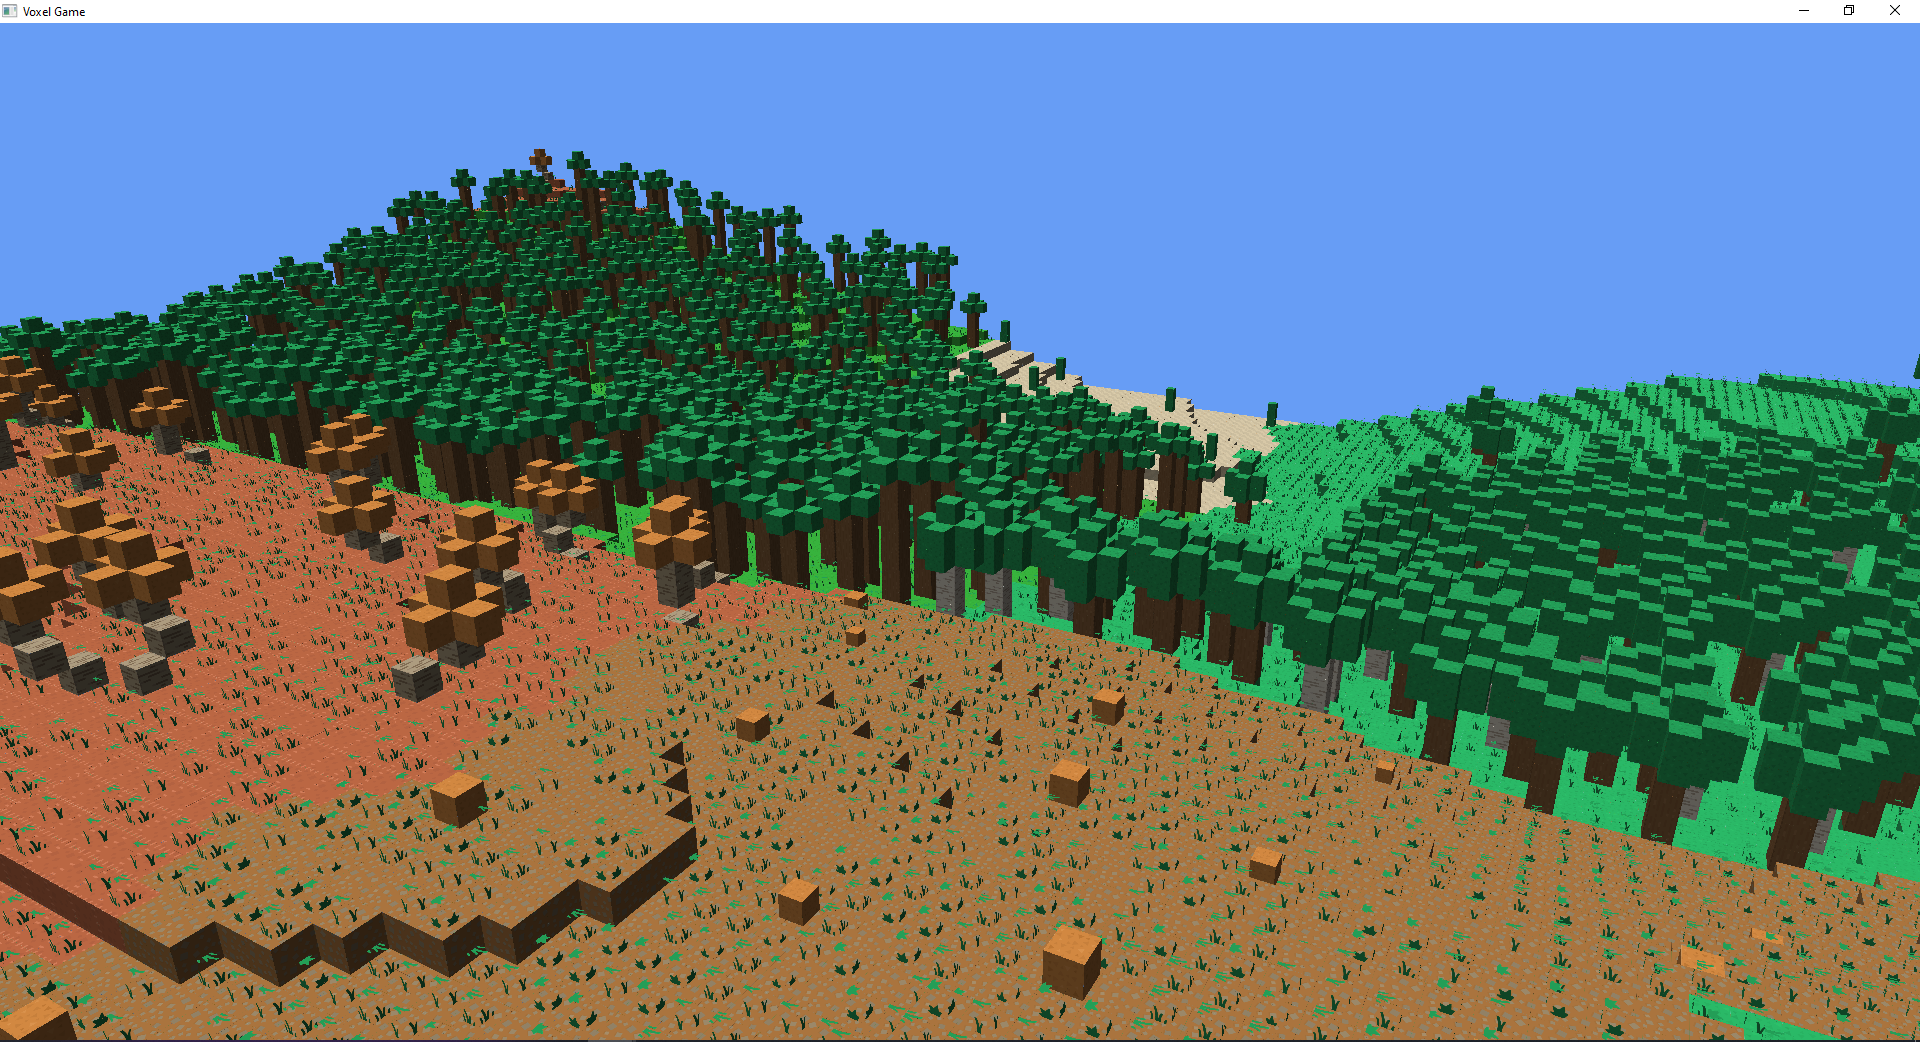
\includegraphics[width=\textwidth]{images/identical_trees}
	\caption[Identické stromy]{Identické stromy}\label{fig:identicke_stromy}
\end{figure}

\section{L-systém}
L-systém nebo také Lindenmayerův systém je paralelní přepisovací systém vyvinutý maďarským teoretickým biologem a botanistou Aristidem Lindenmayerem v roce 1968. L-systém je typ formální gramatiky skládající se z abecedy, přepisovacích pravidel a počátečního axiomu. Pomocí postupného derivování počátečního axiomu je možné simulovat vývoj rostliny v čase \cite{pcgbook75}.

\section{Interpretace řetězců pomocí želvy}
Řetězce lze graficky reprezentovat pomocí želvy, konsumující symboly abecedy. Každý symbol určuje akci, kterou má želva vykonat. Želva se může pohybovat ve 2D nebo 3D prostoru. Ve 2D si můžeme interpretaci představit jako želvu, držící tužku, pohybující se po papíře.

Želvu lze reprezentovat jako trojici $(x, y, \alpha)$, kde $(x, y)$ představuje kartézské souřadnice reprezentující polohu v prostoru a $\alpha$ úhel kam želva směřuje. Zadáním délky kroku \textit{d} a změny úhlu $\delta$ lze želvu ovládat pomocí následujících symbolů.

\begin{itemize}
\item F -- Posun dopředu o délku $d$. Stav želvy se změní na $(x’, y‘, \alpha)$, kde $x = x + d \cos \alpha$ a $y = y + d \sin \alpha$. Mezi body $(x, y)$ a $(x’, y‘)$ je nakreslena čára.
\item + -- Rotace doleva o úhel $\delta$. Nový stav želvy $(x, y, \alpha + \delta)$.
\item - -- Rotace doprava o úhel $\delta$. Nový stav želvy $(x, y, \alpha - \delta)$.
\end{itemize}

Nechť je definován následující L-systém. Buď $\omega$ počáteční axiom, $p$ přepisovací pravidlo, $\delta = 90\degree$ a $d$ zmenšené čtyřnásobně pro každý obrázek~\cite{abop7}.

\bigskip
$\omega: F-F-F-F$

\medskip
$p: F \rightarrow F-F+F+FF-F-F+F$

\bigskip
Želva interpretující daný L-systém generuje kvadratické Kochovy ostrovy~\ref{fig:koch_island}. Obrázky jsou vygenerovány derivacemi o délce 0 až 3.

\begin{figure}\centering
	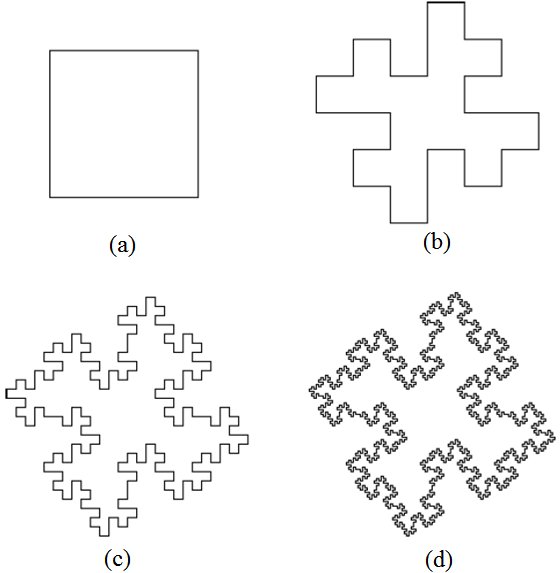
\includegraphics[width=\textwidth]{images/koch_island}
	\caption[Kvadratické Kochovy ostrovy]{Kvadratické Kochovy ostrovy}\label{fig:koch_island}
\end{figure}

\section{Větvení v L-systémech}
S danými přepisovacími pravidly není možné generovat větvící se struktury. Želva vždy pokračuje od své poslední pozice. Říše rostlin je dominovaná větvícími se strukturami, potřebujeme proto matematické vyjádření této skutečnosti.

Větvení v řetězci můžeme reprezentovat pomocí dvou symbolů [ a ], kde [ značí začátek větve a ] konec větve~\cite{abop24}.

Symboly jsou interpretovány želvou následovně:

\begin{itemize}
\item $[$ -- Ulož atributy želvy do zásobníku.
\item $]$ -- Načti atributy želvy ze zásobníku a smaž je z vrcholu zásobníku (operace pop). Při této operaci není nakreslená žádná čára.
\end{itemize}

Díky nově přidaným symbolům lze generovat struktury připomínající rostliny. Struktury na obrázku~\ref{fig:plant_like_str} jsou generované následujícími L-systémy:

\begin{enumerate}
\item $\delta = 20\degree$

	$\omega: E$
	
	$p1: F \rightarrow FF$
	
	$p2: E \rightarrow F[+E]F[-E]+E$
	
\item $\delta = 25,7\degree$

	$\omega: E$
	
	$p1: F \rightarrow FF$
	
	$p2: E \rightarrow F[+E][-E]FE$

\end{enumerate}

L-systém 1 generuje rostlinu vlevo, L-systém 2 generuje rostlinu vpravo.

\begin{figure}\centering
	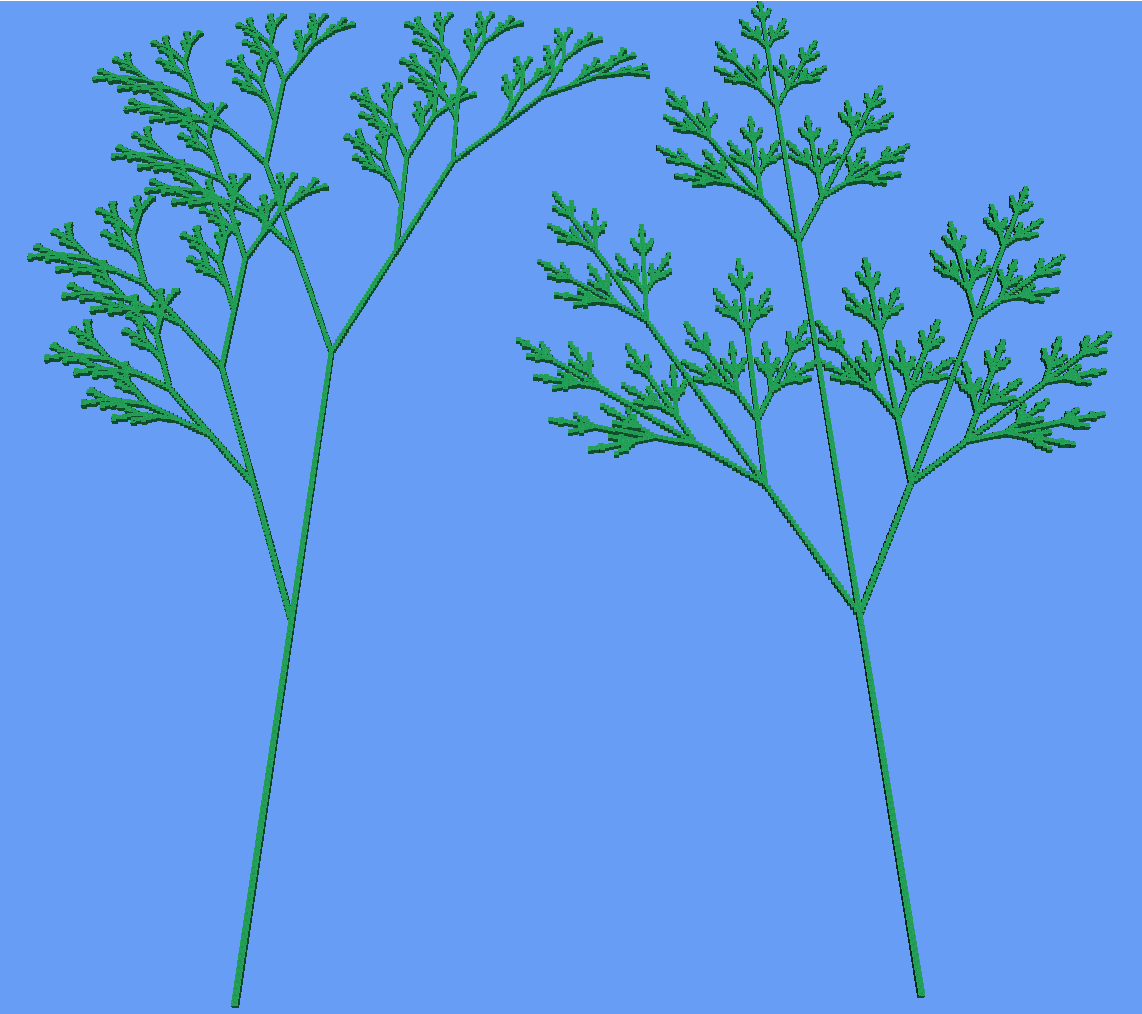
\includegraphics[width=\textwidth]{images/plant_d_e}
	\caption[Struktury připomínajících rostliny]{Struktury připomínajících rostliny generované pomocí závorkovaného systému}\label{fig:plant_like_str}
\end{figure}

\section{Stochastické L-systémy}
Rostliny generované deterministickým L-systémem jsou všechny stejné. Jejich použití v scéně by vytvářelo stejný efekt, který je popsán na začátku kapitoly. 

K předejití tohoto efektu je nutné zavést variace v rámci druhu. Náhodná interpretace řetězce má limitované využití. Změna úhlu větvení, šířky a výšky segmentů rostliny zachovávají topologii struktury, ze které je generovaná. Stochastické L-systémy mohou měnit topologii struktury~\cite{abop28}.

-systém, který byl do teď používán nemohl mít více přepisovacích pravidel pro stejný symbol abecedy. Pokud má stochastický L-systém vice přepisovacích pravidel, je z nich vybrána jedna s pravděpodobností $1/n$, kde $n$ je počet přepisovacích pravidel pro daný symbol abecedy
\footnote{Tato definice se liší, od definice uvedené ve~\cite{abop28}. Tento způsob náhodného výběru je použit v implementaci, kde pravděpodobností distribuci zastupuje několikanásobné zopakování přepisovacího pravidla.}.

Scéna~\ref{fig:plant_stoch} byla vygenerována za pomocí stochastického L-systému, kde:

\bigskip 
$\delta = 25,7\degree$

\medskip
$\omega: F$

\medskip
$p1: F \rightarrow F[+F]F[-F]F$

\medskip
$p2: F \rightarrow F[+F]F$

\medskip
$p3: F \rightarrow F[-F]F$

\begin{figure}\centering
	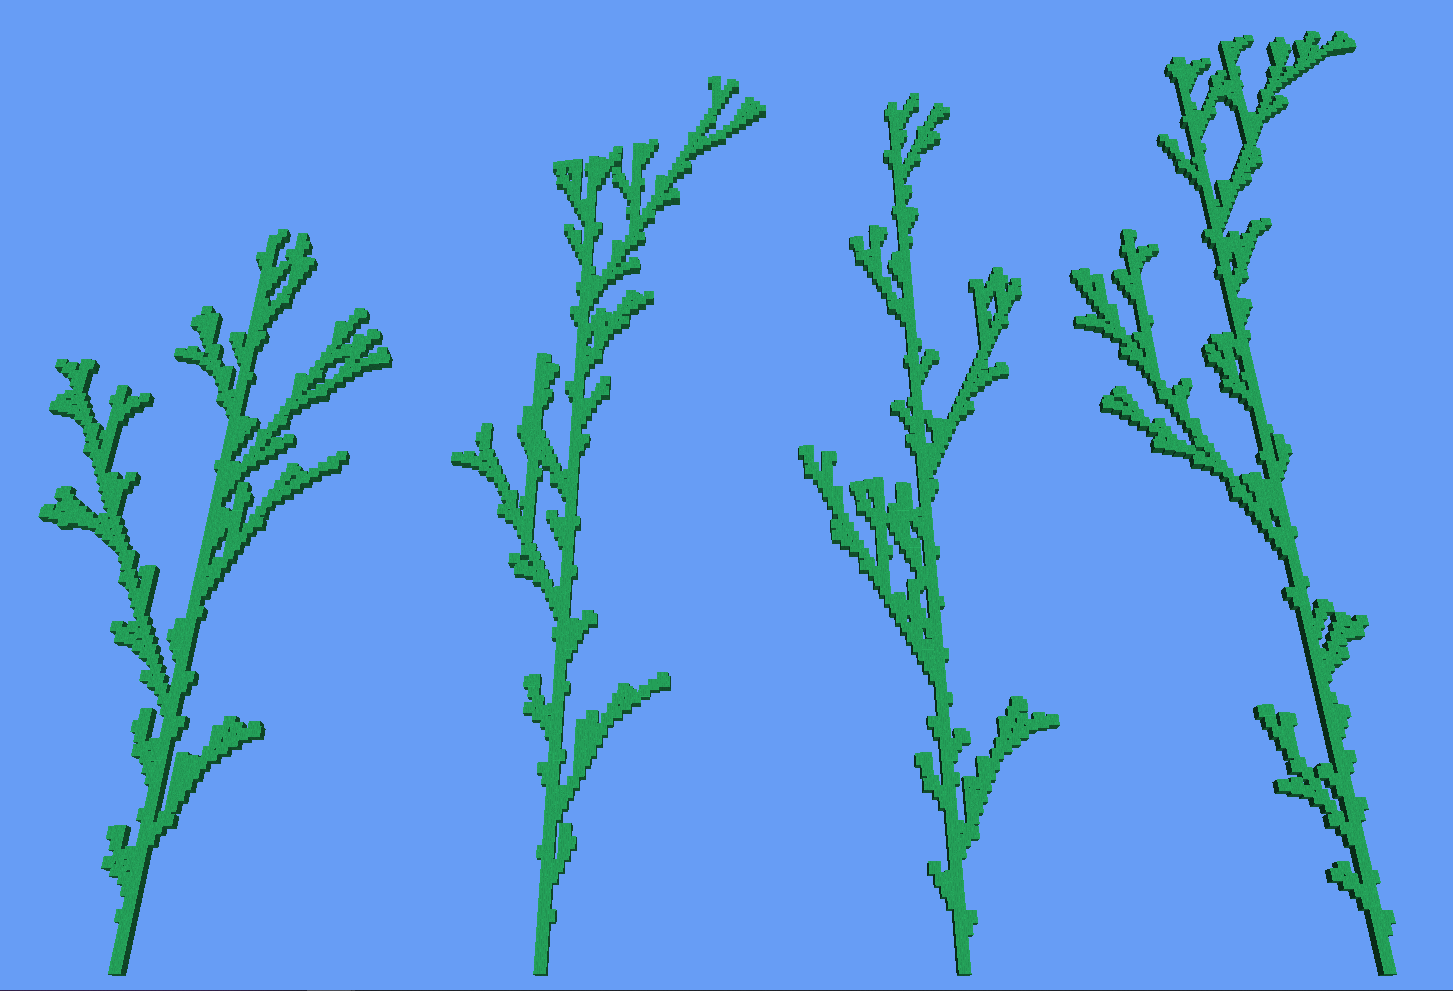
\includegraphics[width=\textwidth]{images/plant_stoch}
	\caption[Využití stochastického L-systému]{Využití stochastického L-systému}\label{fig:plant_stoch}
\end{figure}

\section{Implementace}
\subsection{Formát L-systému}

L-systém může být načten ze souboru pomocí třídy \texttt{LSystemParser}. L-systém musí mít následující formát:

\begin{verbatim}
yaw_angle pitch_angle shring_ratio
axiom
letter > production
.
.
.
letter > production
\end{verbatim}

Soubor může obsahovat za sebou jdoucí L-systémy. \texttt{LSystemParser} je vrátí jako pole. Soubor může obsahovat komentáře na nových řádcích, začínající symbolem \#.

Třída \texttt{LSystem} obsahuje gramatiku a tři atributy specifikující úhel náklonu podle osy y (yaw), podle osy x (pitch) a změnu velikosti bloku. Poslední atribut je využit při rozvětvení rostliny. Potomci mateřské větve by se měly řídit postulátem Leonarda da Vinci: „všechny větve stromu, v každé úrovni jeho růstu jsou v součtu jejich tloušťky rovné tloušťce kmene pod nimi.“ V případě dvojitého rozvětvení, tloušťky mateřské větve $w_1$, tloušťky potomků $w_2$ dostaneme rovnici~\cite{abop57}:

\[ w_1^2 = 2w_2^2 \]
\[ \frac{w_2}{w_1} = \frac{1}{\sqrt{2}} \approx 0,707\]

Hodnotu 0,7 je možné nalézt v L-systémech modelující keře.

\subsection{Želva}
Třída \texttt{Turtle} rozšiřuje pohyb želvy –- popsané v kapitole Interpretace řetězců pomocí želvy –- do 3D prostoru. Vnitřní stav želvy určují následující atributy:

\begin{itemize}
\item Pozice v prostoru.
\item Velikost bloku vytvořeného želvou.
\item Barva použitá pro kreslení (výstupní pole).
\item Yaw –- rotace podle osy y.
\item Pitch –- rotace podle osy x.
\end{itemize}

Želva si udržuje tři navzájem kolmé směrové vektory (nahoru, dopředu, doprava) jednotkové délky, které využívá pro pohyb po scéně. Vektory jsou aktualizované po každé rotaci. Pro výpočet je nutné znát vektor směrující kolmo vzhůru vůči scéně (\texttt{WORLD\_UP}). Generovaný svět je plochý, proto lze tento vektor nahradit konstantním vektorem $(0, 1, 0)$.

\begin{verbatim}
glm::vec3 front;
front.x = cos(glm::radians(Yaw_)) * cos(glm::radians(Pitch_));
front.y = sin(glm::radians(Pitch_));
front.z = sin(glm::radians(Yaw_)) * cos(glm::radians(Pitch_));

Front_ = glm::normalize(front);
Right_ = glm::normalize(glm::cross(Front_, WORLD_UP));
Up_ = glm::normalize(glm::cross(Right_, Front_));
\end{verbatim}

Délku \textit{x} v rovině určené osami \textit{x} a \textit{z} lze spočítat jako délku přilehlé odvěsny. $\cos(Yaw) = x / h$, kde \textit{h} je délka přepony. Víme, že vektor má jednotkovou délku, proto $h = 1$. Stejný postup aplikujeme pro rovinu určenou osami \textit{x} a \textit{y}.

Tímto způsobem dopočítáme délky \textit{y} a \textit{z} vektoru směrujícího dopředu a normalizujeme ho. Jelikož jsou na sebe vektory kolmé, využijeme vektorového součinu, jehož výsledkem je vektor kolmý k oběma původním vektorům. Všechny vektory je nutné normalizovat, aby se předešlo jejich zkracování s tím, jak se Pitch blíží $\pm 90\degree$.

K zamezení převrácení os jsou z definičního oboru Pitch vyjmuty násobky 90\degree.

\begin{verbatim}
if (Helpers::Math::Equal(cos(glm::radians(Pitch_)), 0.0f))
    Pitch_ -= 0.01f;
\end{verbatim}

Výsledná nepřesnost je menší než maximální rozdíl dvou čísle typu float~$\epsilon$, která jsou považována za stejná. Funkce \texttt{Equal} porovnává desetinná čísla s přesností~$\epsilon$.

Želva vystavuje metody pro pohyb ve všech třech osách využívající vektorů \texttt{Up\_, Right\_, Forward\_}. K pozici želvy je přičten patřičný vektor naškálovaný délkou pohybu. Např.:

\begin{verbatim}
void LSystems::Detail::Turtle::MoveForward(float dz) {
    Position_ += Front_ * dz;
}
\end{verbatim}

\subsection{Rozšířená abeceda}
Následující symboly abecedy mají speciální význam pro jejich interpretaci.

\begin{itemize}
\item U a u –- Posuň želvu nahoru.
\item F a f –- Posuň želvu dopředu.
\item x –- Zmenši želvu.
\item X –- Zvětši želvu.
\item S –- Nastav původní velikost želvy.
\item + –- Rotuj želvu doleva podle osy y.
\item - –- Rotuj želvu doprava podle osy y.
\item $\hat{}$ –- Rotuj želvu nahoru podle osy x.
\item \& –- Rotuj želvu dolů podle osy x.
\item $[$ –- Ulož kopii želvy na vrchol zásobníku.
\item $]$ –- Vyjmi želvu z vrcholu zásobníku.
\item $0-9$ –- Přepni výstupní pole.
\end{itemize}

L-systém může obsahovat jakýkoliv jiný ASCII symbol –- mimo bílých znaků a \# –- určený pro expanzi přepisovacích pravidel. Není želvou interpretován.

\subsection{Ovládání želvy}
Implementace želvy se nachází ve jmenném prostoru \texttt{LSystems::Detail}, uživatel by ji neměl využívat přímo, ale je pro něj připravena třída \texttt{LSystemExecutor} zajišťující generování herních objektů z poskytnutého L-systému.

\texttt{LSystemExecutor} umožňuje generovat herní objekty na základě stochastického L-systému –- topologie struktury výsledného modelu se může měnit mezi jednotlivými voláními generátoru na základě parametru \texttt{salt}. L-systém lze náhodně interpretovat na základě těchto parametrů:

\begin{itemize}
\item Rozsah počtu provedených derivací.
\item Variace v rotaci želvy. K úhlu, o který se má želva otočit, se přičte x * původní úhel, kde x je z [-angleVar, angleVar]. Defaultní hodnota angleVar je 0,2.
\item Výchozí velikost generovaných objektů. Lze určit rozsahem korespondujícím s počtem derivací.
\end{itemize}

Přidání náhodného úhlu má výrazný efekt na organický vzhled rostliny. Na obrázku~\ref{fig:acacia_random_angle_leaves} lze vidět akáciové stromy vyznačující se plochou korunou. V definici L-systému jsou všechny listy ve stejné výšce, výsledný rozdíl ve výškách je způsoben opakovaným rotováním želvy. V zápisu lze vidět, že se želva otočí o 45\degree nahoru (~$\hat{}$~), pokládá větve (u, U), skloní se o 45\degree (\&) a pokládá listy (F). Listy by tak měly být ve stejné rovině, ale nejsou.

L-systém generující akácie:

\begin{verbatim}
45.0 45.0 0.8
# make sure the plant has splits
# random lenght stem - then split
^uA1S&F+F+F+F
U > uU
A > +uuE
A > -uE
A > +uE
A > -E
A > uuE
A > uE
# top of the plant
E > x[++++UE1S&F+F+F+F]+UE
E > x[++++++UE1S&F+F+F+F]++UE
E > x[++UE1S&F+F+F+F]-UE
\end{verbatim}

\begin{figure}\centering
	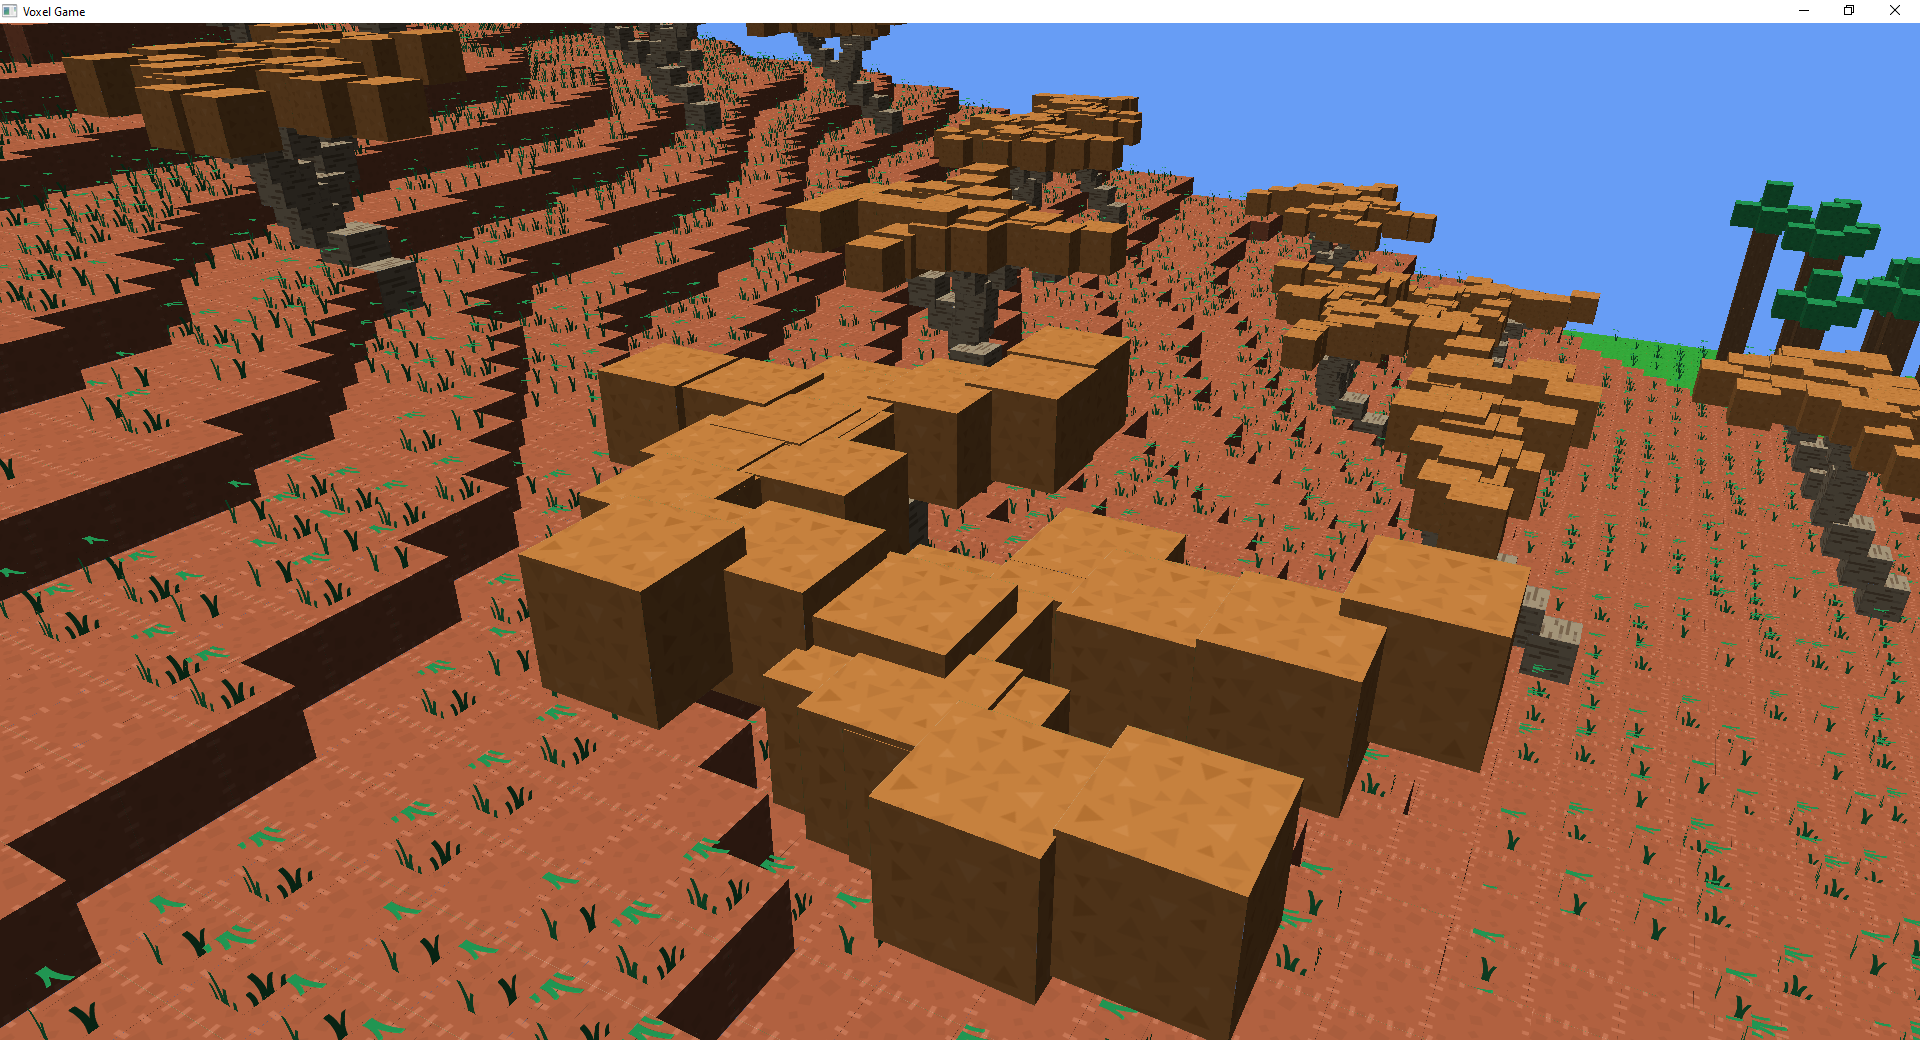
\includegraphics[width=\textwidth]{images/acacia_random_angle_leaves}
	\caption[Nepravidelná koruna akáciového stromu]{Nepravidelná koruna akáciového stromu}\label{fig:acacia_random_angle_leaves}
\end{figure}

Výstupem generátoru je 2D pole obsahující herní objekty rozdělené podle čísla výstupního bufferu, který měla želva při generování. Část enginu je tak odstíněna od textur, které jsou definované v~části procedurálního generátoru. Díky tomuto rozdělení modelu je možné snadno měnit textury pro jednotlivá pole. Procedurální generátor tohoto využívá a~používá stejný model -- jiný běh generátoru -- pro vytváření bříz a~dubů, lišících se texturou kmene a listů.

\section{Modelování rostlin}

Při modelování vegetace bylo třeba velkého množství pokusů a~ladění, kdy rostlina nevypadala přirozeně, ale nebylo jasné, v jaké časti gramatiky je problém. Nejvíce se mi osvědčila technika nalezení reálné rostliny obrázek~\ref{fig:acacia_nature} a~následné pokusy o její napodobení obrázek~\ref{fig:acacia_engine}.

Velice se osvědčilo pravidlo:

\begin{verbatim}
U > uU
\end{verbatim}

Díky němuž jsou větve blíže k zemi delší než větve navazující na korunu stromu. Pokud má rostlina význačné části je vhodné je modelovat samostatně (kmen, větve, koruna) viz L-systém generující akácie.

\begin{figure}\centering
	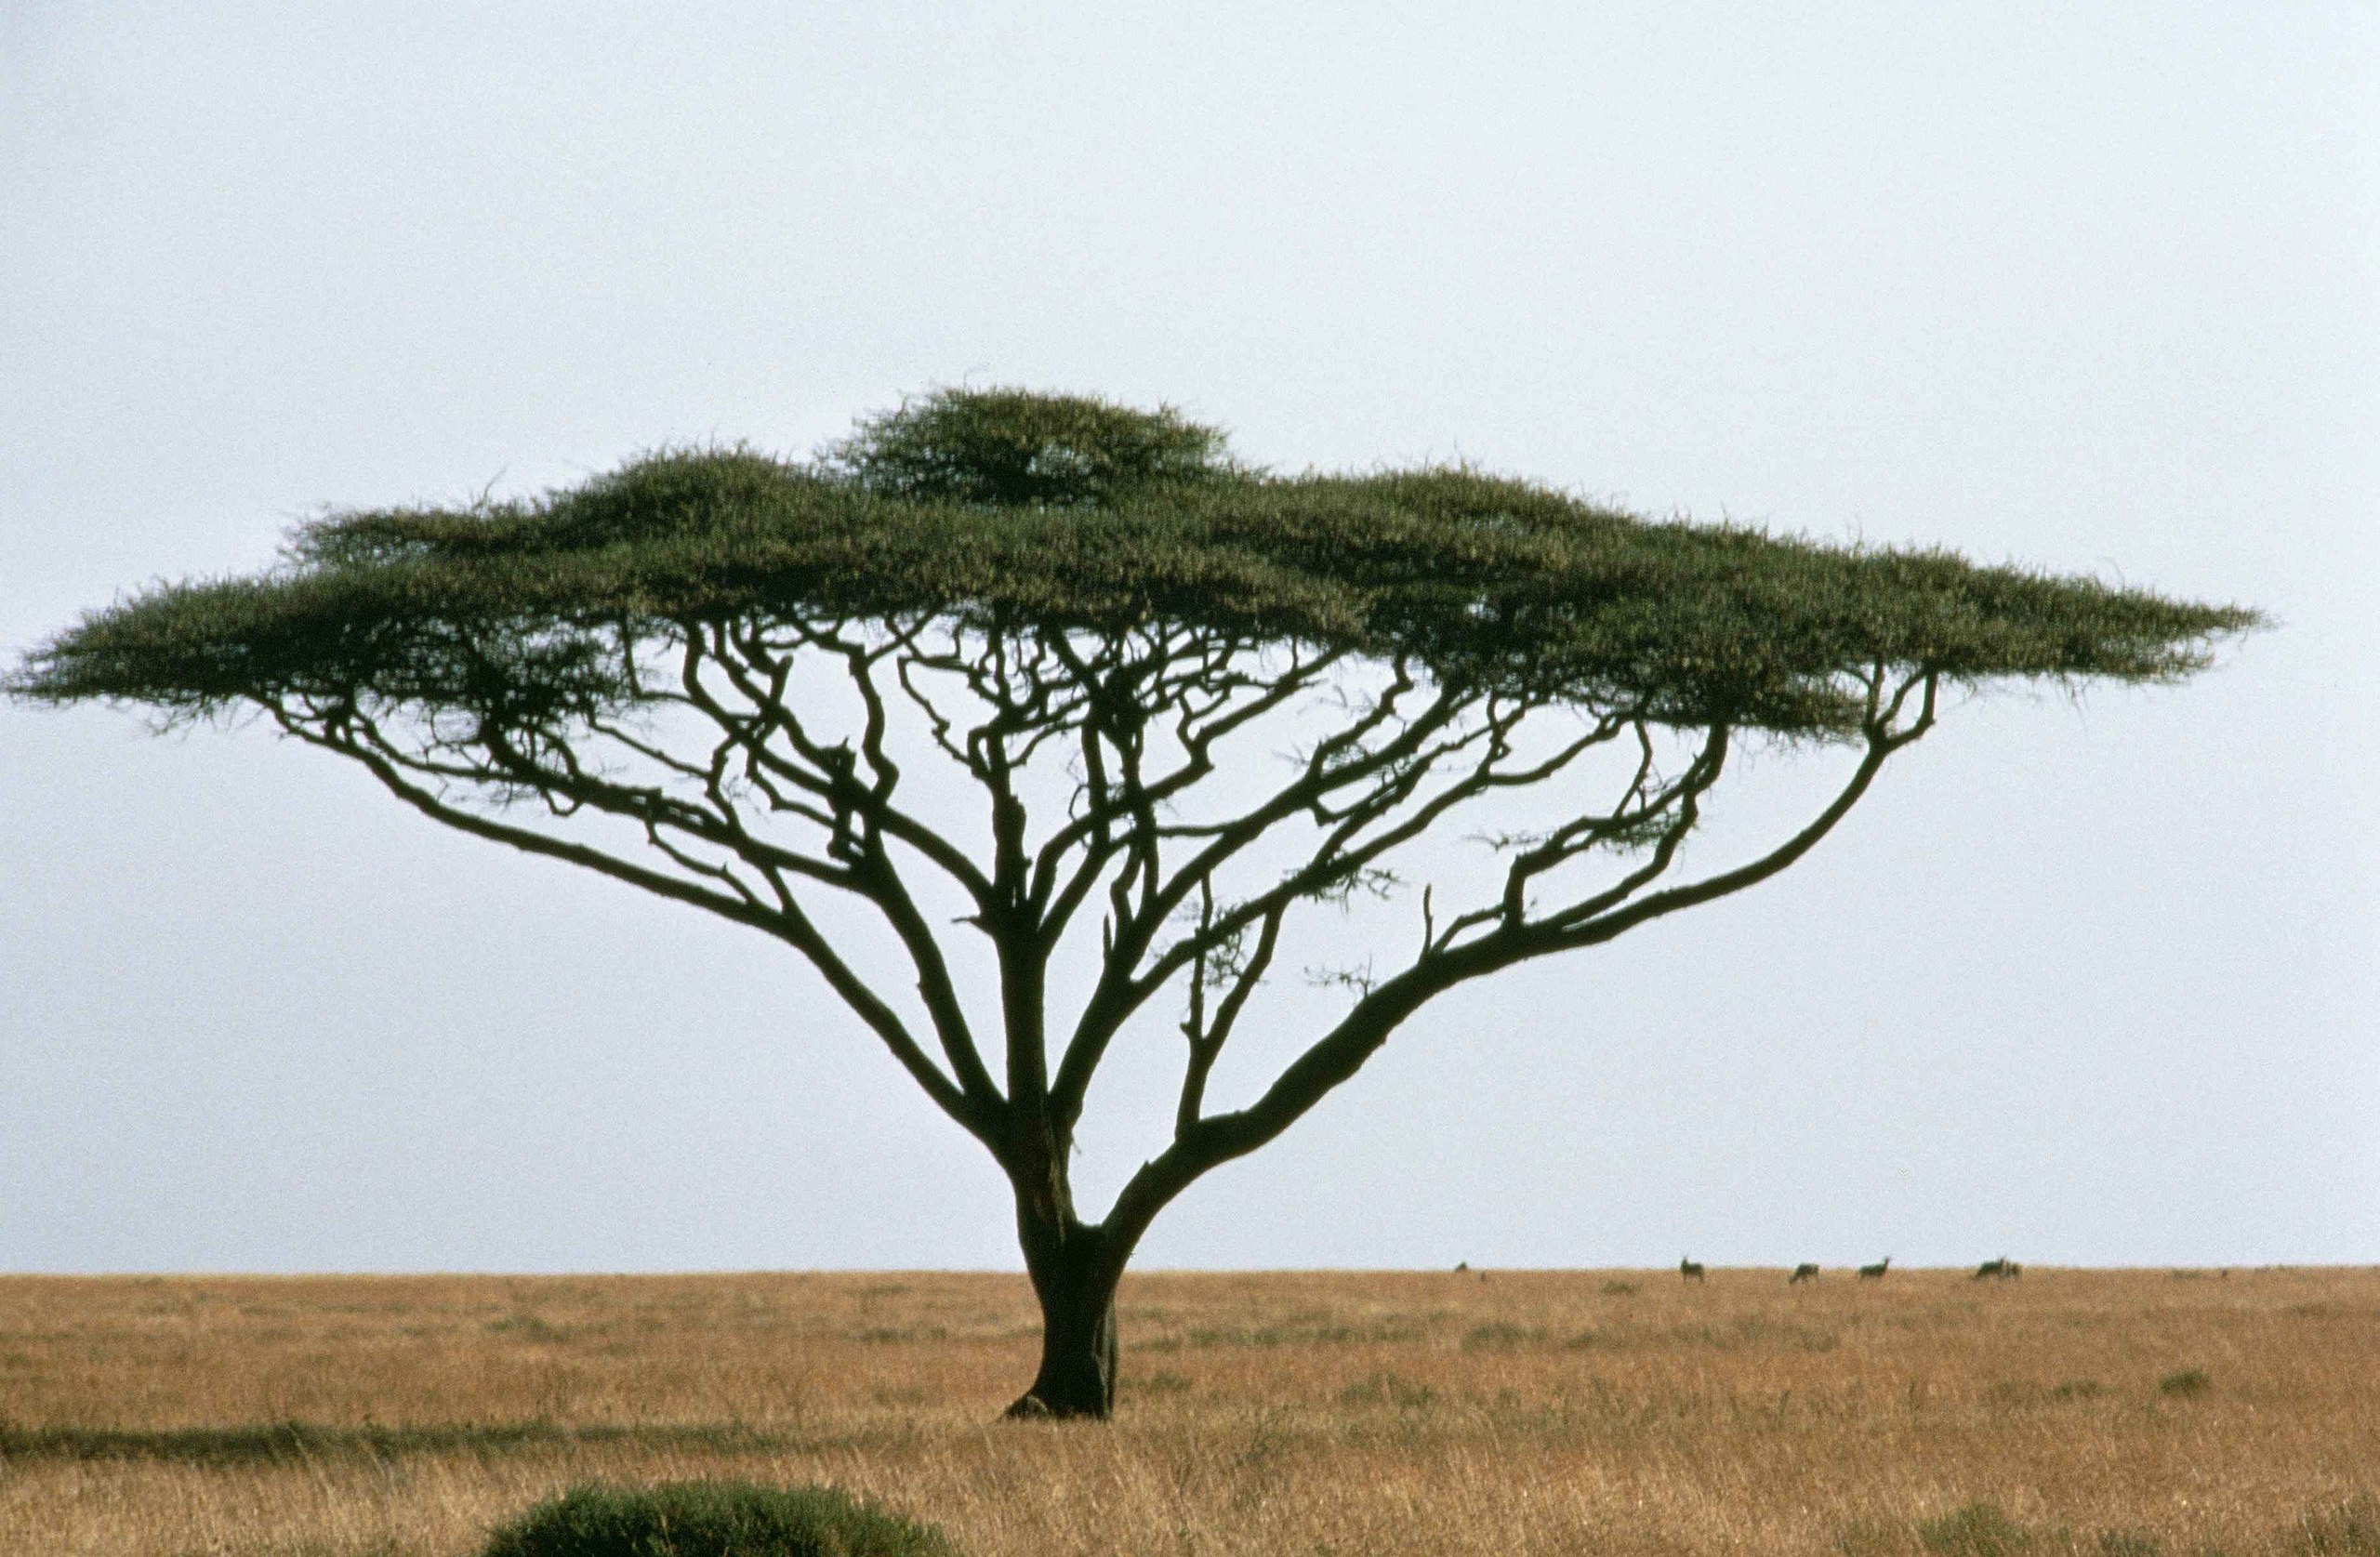
\includegraphics[width=\textwidth]{images/acacia_nature}
	\caption[Akáciový strom rostoucí v přírodě]{Akáciový strom rostoucí v přírodě~\cite{acacia}}\label{fig:acacia_nature}
\end{figure}

\begin{figure}\centering
	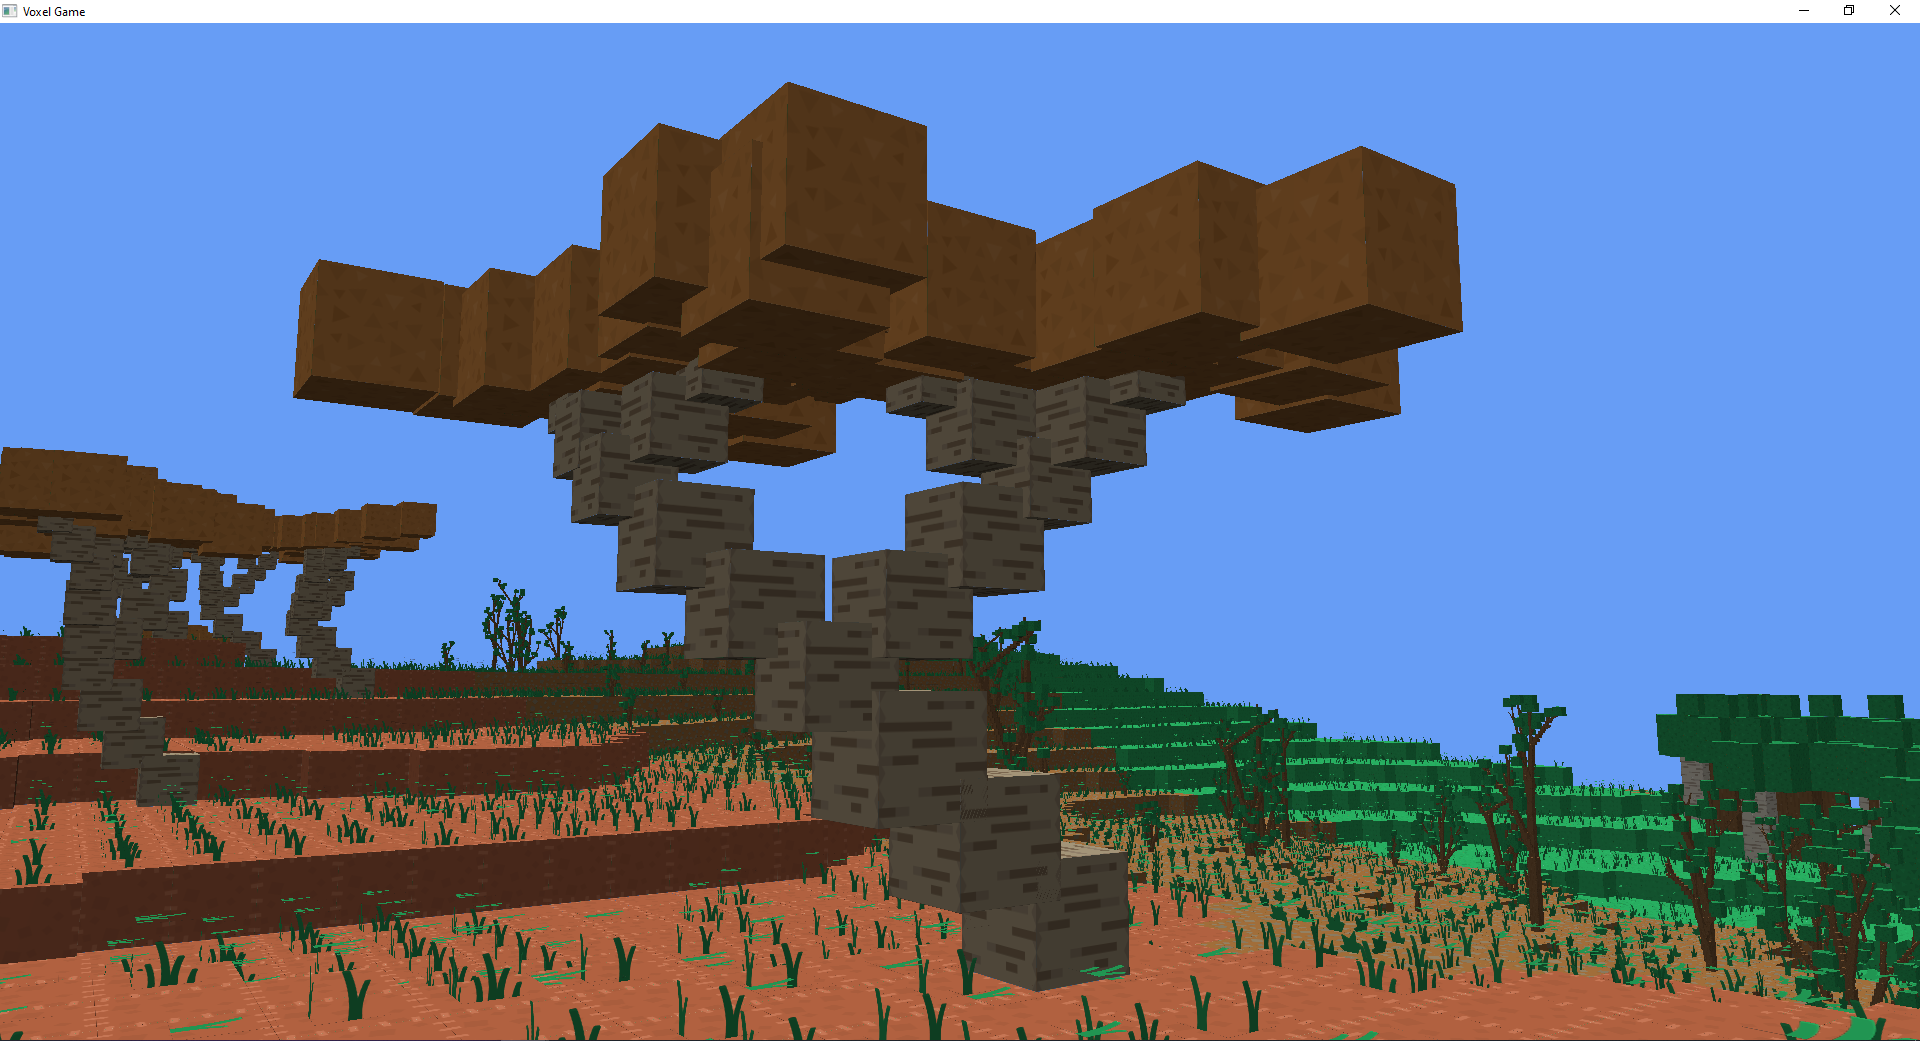
\includegraphics[width=\textwidth]{images/acacia_engine}
	\caption[Model akáciového stromu]{Model akáciového stromu}\label{fig:acacia_engine}
\end{figure}

Tato technika ne vždy přinášela ovoce. Modelování trávy rostoucí na planinách se projevilo jako problém. Tráva neměla dostatečnou hustotu a nezapadala do kresleného vzhledu obrázek~\ref{fig:grass_plains}. S navyšujícím se počtem herních objektů dramaticky rostla spotřeba paměti. Jeden herní objekt s texturou trávy byl nahrazen desítkami herních objektů, z kterých se skládal model trávy. Tento problém by mohl být řešen přesunem vytváření modelu na grafickou kartu, přidáním vertexů v geometry shaderu.

\begin{figure}\centering
	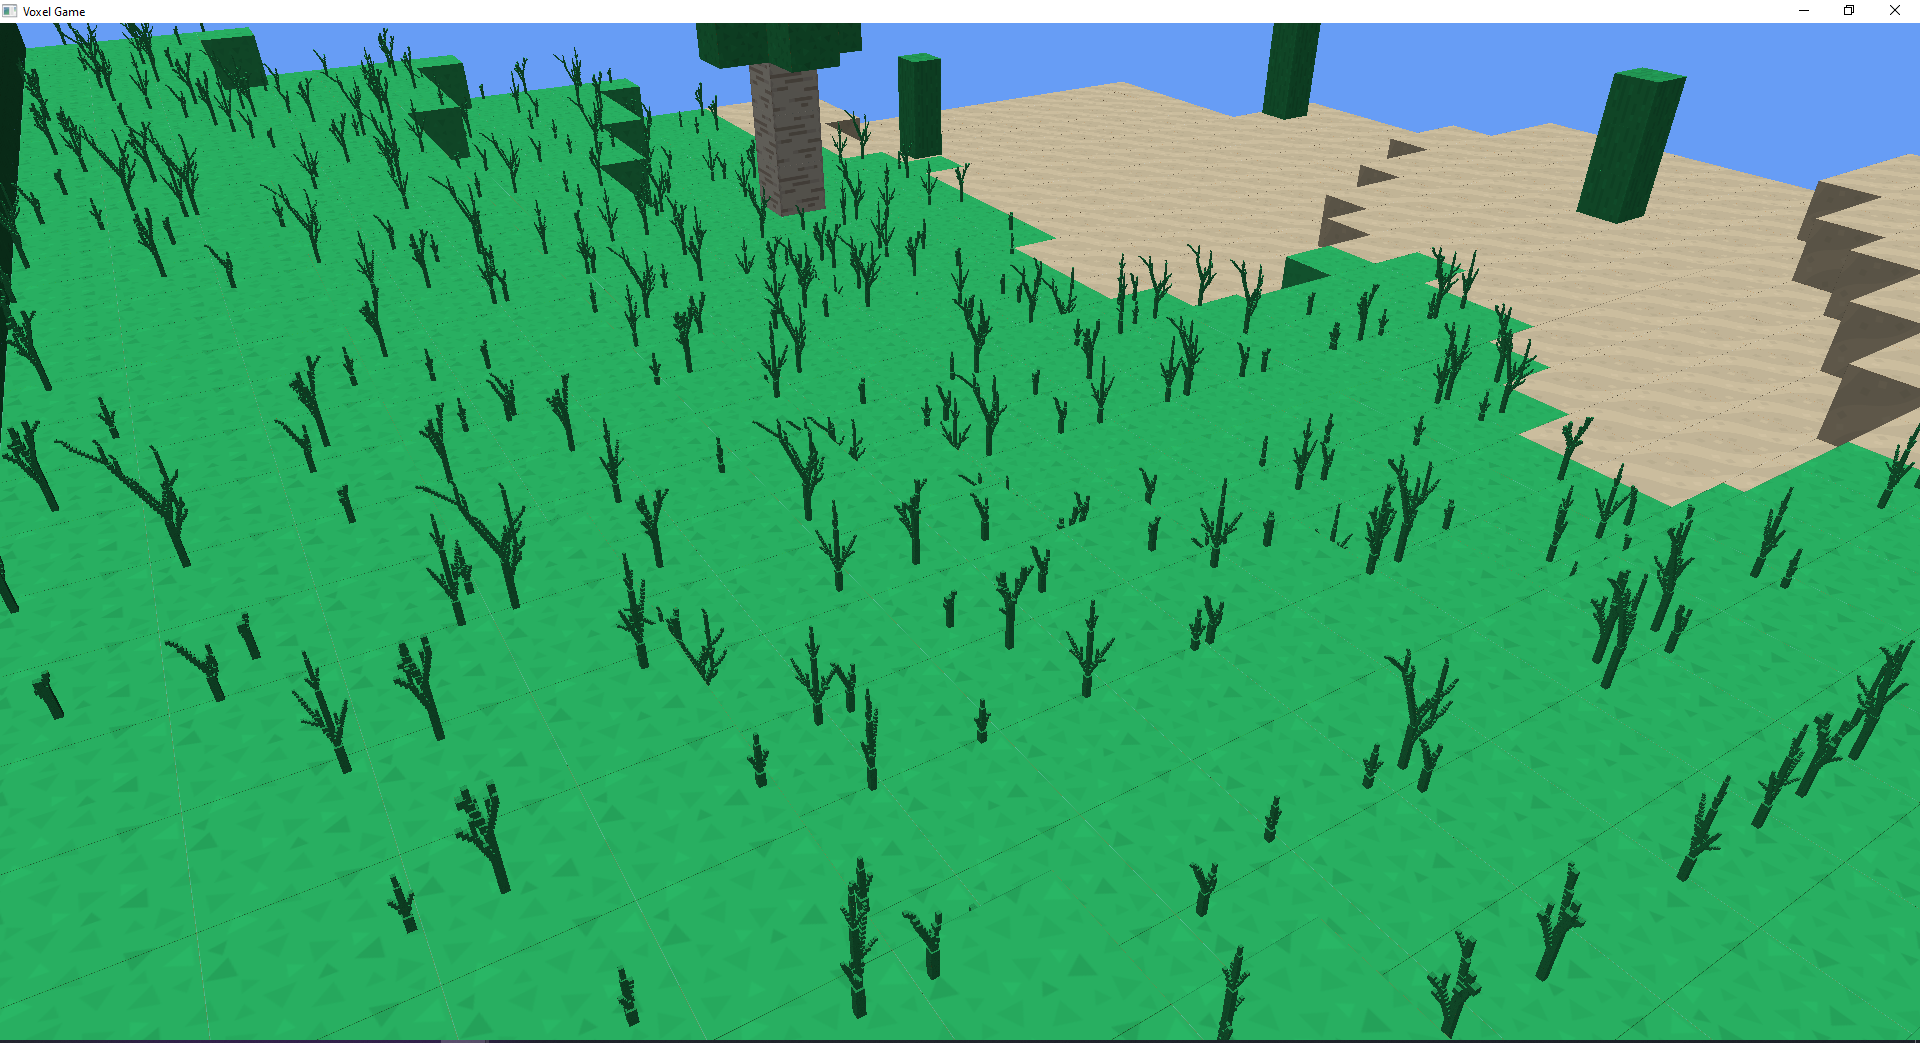
\includegraphics[width=\textwidth]{images/grass_plains}
	\caption[Tráva na planinách]{Tráva na planinách}\label{fig:grass_plains}
\end{figure}

Výsledné modely svou topologií připomínaly strukturu keřů. Byly proto upraveny –- přidáním listí, změnou větvení –- a využity v generátoru keřů.

\subsection{Simulace růstu}
Křovinatý biotop je porostlý dvěma druhy keřů rozděleným do třech fází růstu. Ty jsou simulovány opakovaným derivováním počátečního axiomu. Keře nejmenšího vzrůstu jsou derivovány 2x, největší keře jsou derivovány 4x. Tloušťka kmene koreluje lineárně s počtem provedených derivací. Větší stromy mají širší kmen a dorůstají vyšší výšky.

Každý druh si zachovává své typické vlastnosti. Na obrázku~\ref{fig:shrub_evolution}\footnote{Pro větší názornost byly odstraněny části modelu představující listy.}  lze pozorovat stejné zakončení větví –- rozdělení do dvou větví rostoucích na opačné strany –- a~podobný úhel v~jakém se větve oddělují od kmene. Topologie rostliny se díky stochastickému L-systému mění mezi jednotlivými jedinci.

\begin{figure}\centering
	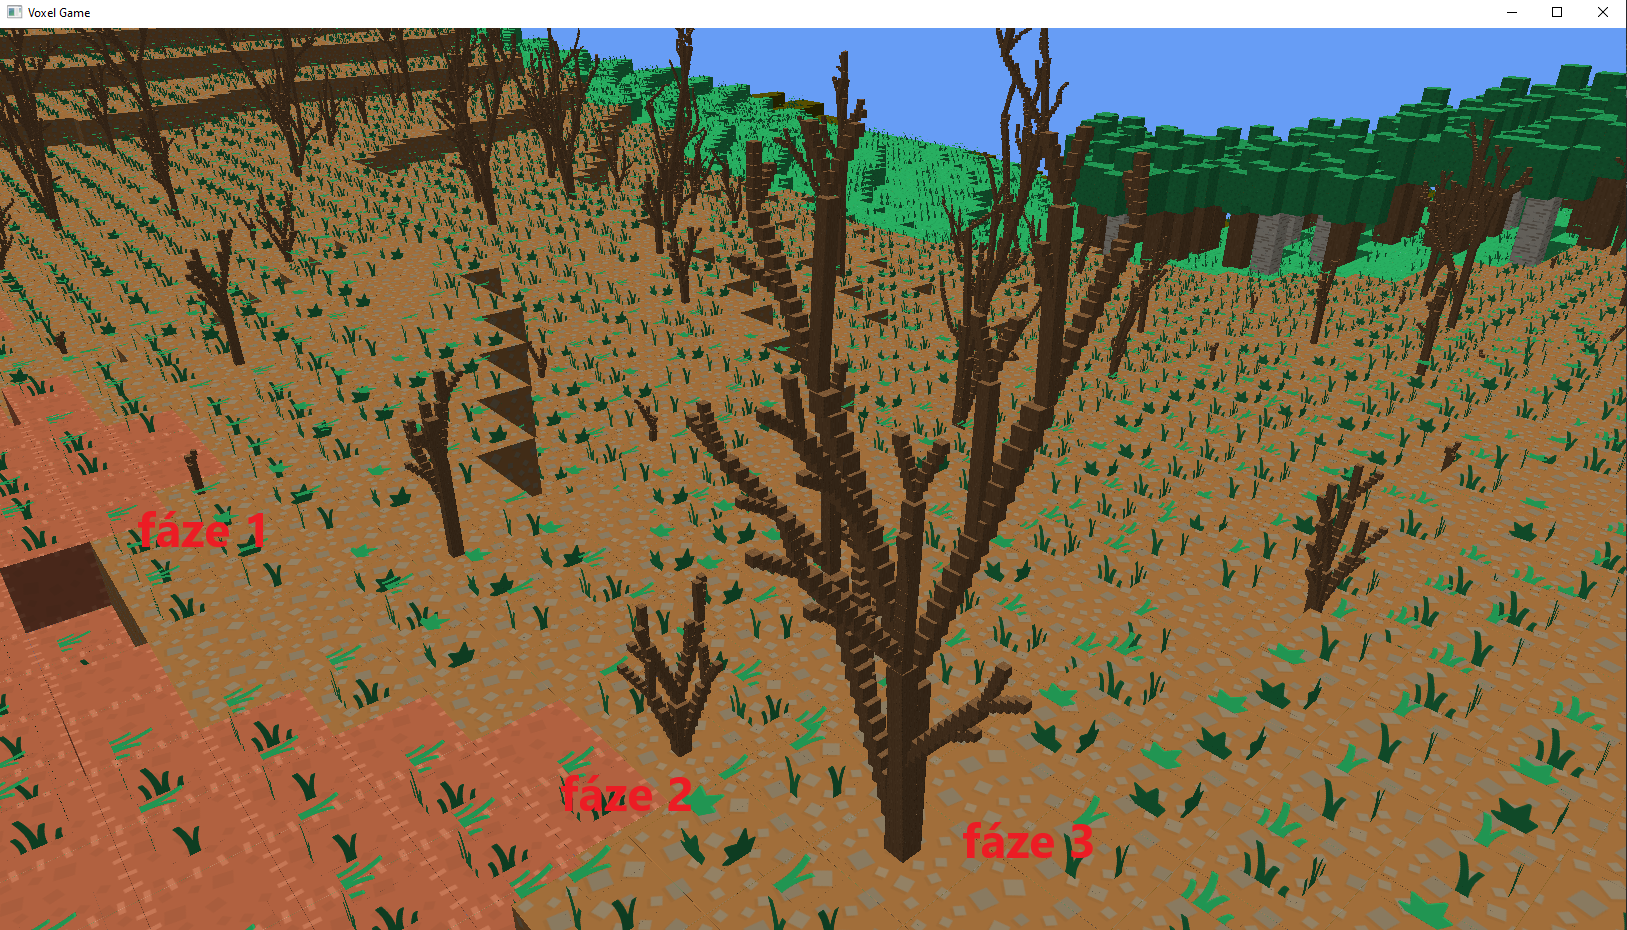
\includegraphics[width=\textwidth]{images/shrub_evolution}
	\caption[Fáze růstu keře]{Fáze růstu keře}\label{fig:shrub_evolution}
\end{figure}

Díky těmto krokům biotop obsahuje rostliny navzájem podobného vzhledu, lišících se v~drobných detailech.

\section{Výsledky použití L-systémů}
Definice L-systémů jsou krátké ($\approx$10 řádků na jeden druh rostliny) a produkují velké množství rozdílných jedinců. Předchozí manuální definování rostlin v kódu bylo náročnější, a i při přidání více jedinců pro každý druh, by bylo snadné najít stejné. Odebráním definic rostlin z kódu se zvýšila jeho čitelnost –- definice L-systémů jsou zdroje dat, který engine konzumuje. Nutnost kompilace při změně modelu byla odstraněna a zvýšila se rychlost iterace, s kterou je možné upravovat model.

Vytvořením vlastního formátu pro zápis modelu rostliny se oddělila závislost na programovacím jazyce. Modely tak může vytvářet jiný člen týmu bez znalosti programování a překladu kódu.

Generováním rostlin za běhu programu se snížila rychlost jeho běhu. Tento problém lze mitigovat cachováním rostlin obsahujících velké množství herních objektů. Toto bylo provedeno pro keře. Před spuštěním generace terénu je naplněn buffer obsahující keře vygenerované na základě seedu. Buffer musí být dostatečně velký na to, aby nedošlo ke snížení diverzity rostlin. Při vytváření keře na scéně je vybrán náhodný index do bufferu, závislý na pozici keře. Vybraný model je zkopírován a přesunut na dané místo.

Při porovnání scény~\ref{fig:identicke_stromy} ze začátku kapitoly si lze všimnout přirozenějšího vzhledu krajiny. Koruny stromů se mohou překrývat, scéna díky tomu působí více organicky –- stromy v přírodě nemají přesně stanové hranice, kde končí jeden a začíná druhý. Výsledná scenérie~\ref{fig:new_vegetation} působí méně jednolitě díky rozdílným vývojovým stádiím rostlin.

\begin{figure}\centering
	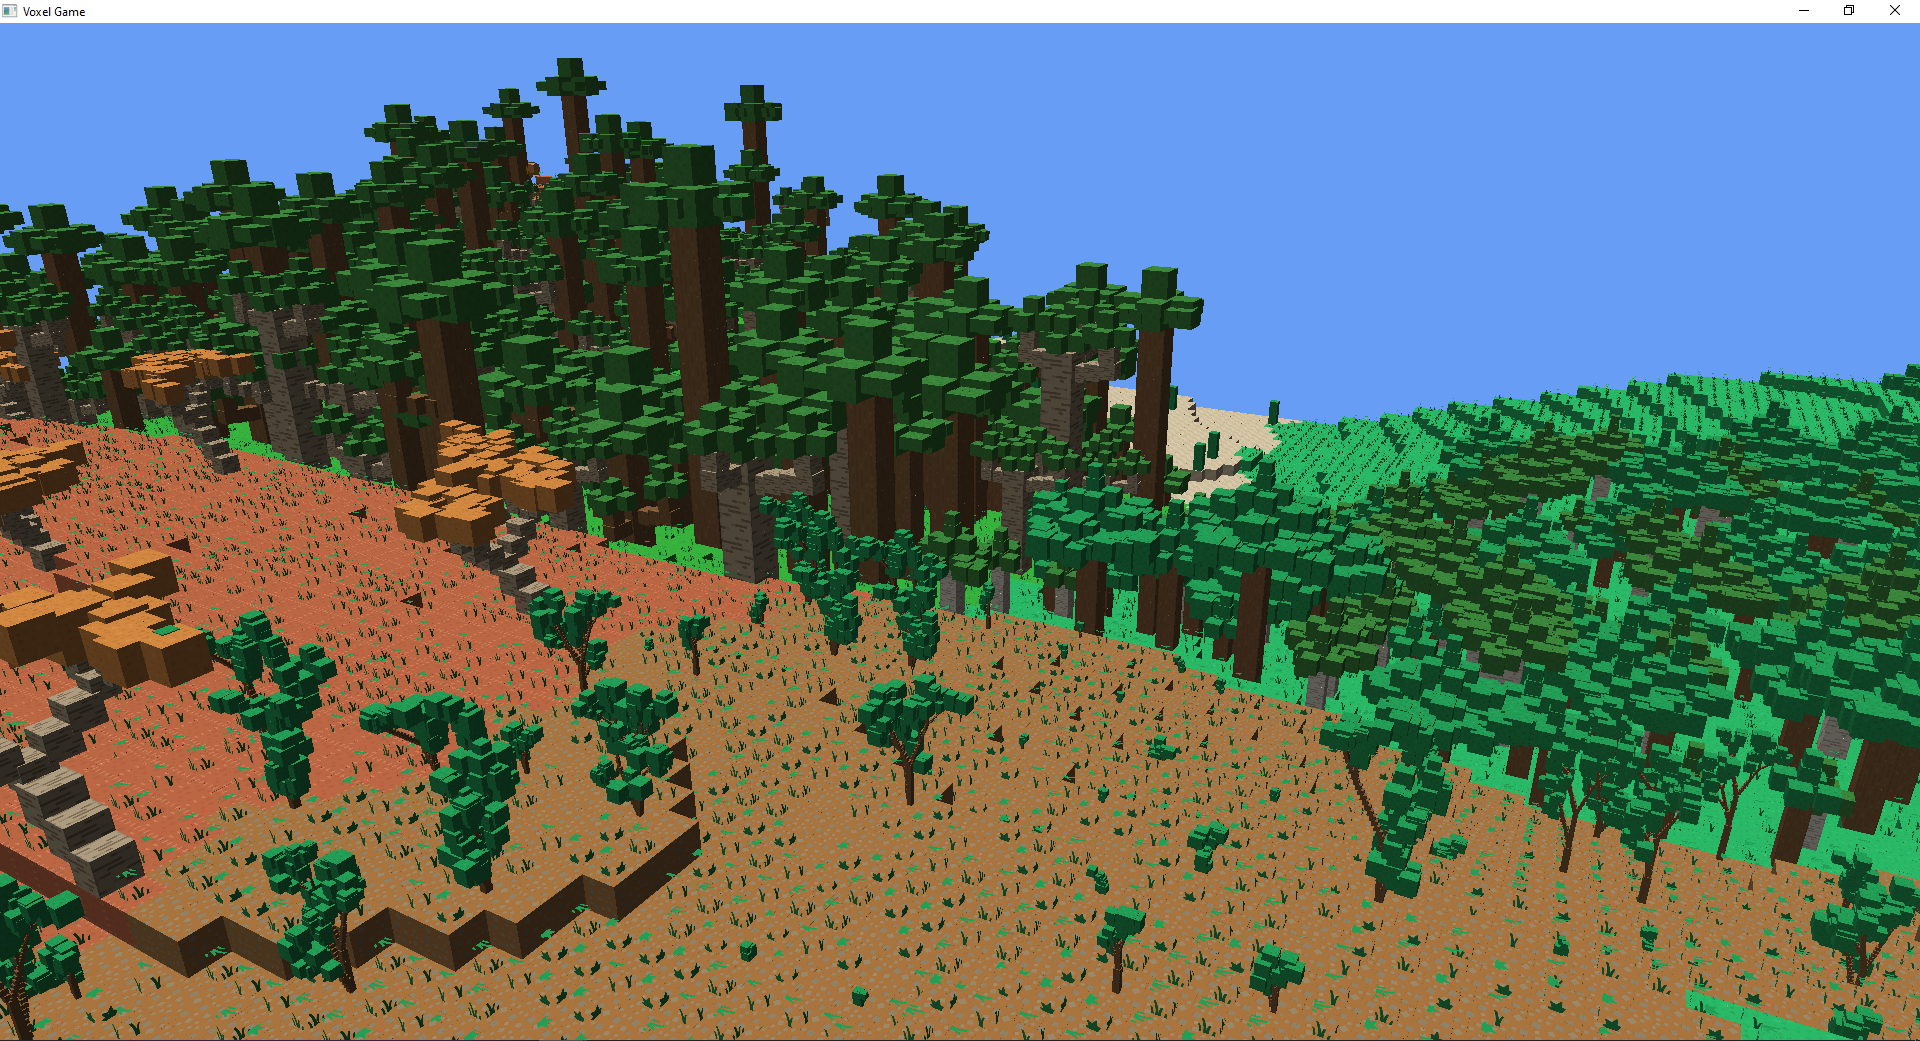
\includegraphics[width=\textwidth]{images/new_vegetation}
	\caption[Vegetace vygenerovaná na základě L-systémů]{Vegetace vygenerovaná na základě L-systémů}\label{fig:new_vegetation}
\end{figure}

% % % % % % % % % % % % % % % % % % % % % % % % % % % % 
% % ZAVER
% % % % % % % % % % % % % % % % % % % % % % % % % % % % 

\begin{conclusion}
	%sem napište závěr Vaší práce
\end{conclusion}

\bibliographystyle{csn690}
\bibliography{mybibliographyfile}

\appendix

\chapter{Seznam použitých zkratek}
% \printglossaries
\begin{description}
	\item[GUI] Graphical user interface
	\item[XML] Extensible markup language
\end{description}


% % % % % % % % % % % % % % % % % % % % % % % % % % % % 
% % Tuto kapitolu z výsledné práce ODSTRAŇTE.
% % % % % % % % % % % % % % % % % % % % % % % % % % % % 
% 
% \chapter{Návod k~použití této šablony}
% 
% Tento dokument slouží jako základ pro napsání závěrečné práce na Fakultě informačních technologií ČVUT v~Praze.
% 
% \section{Výběr základu}
% 
% Vyberte si šablonu podle druhu práce (bakalářská, diplomová), jazyka (čeština, angličtina) a kódování (ASCII, \mbox{UTF-8}, \mbox{ISO-8859-2} neboli latin2 a nebo \mbox{Windows-1250}). 
% 
% V~české variantě naleznete šablony v~souborech pojmenovaných ve formátu práce\_kódování.tex. Typ může být:
% \begin{description}
% 	\item[BP] bakalářská práce,
% 	\item[DP] diplomová (magisterská) práce.
% \end{description}
% Kódování, ve kterém chcete psát, může být:
% \begin{description}
% 	\item[UTF-8] kódování Unicode,
% 	\item[ISO-8859-2] latin2,
% 	\item[Windows-1250] znaková sada 1250 Windows.
% \end{description}
% V~případě nejistoty ohledně kódování doporučujeme následující postup:
% \begin{enumerate}
% 	\item Otevřete šablony pro kódování UTF-8 v~editoru prostého textu, který chcete pro psaní práce použít -- pokud můžete texty s~diakritikou normálně přečíst, použijte tuto šablonu.
% 	\item V~opačném případě postupujte dále podle toho, jaký operační systém používáte:
% 	\begin{itemize}
% 		\item v~případě Windows použijte šablonu pro kódování \mbox{Windows-1250},
% 		\item jinak zkuste použít šablonu pro kódování \mbox{ISO-8859-2}.
% 	\end{itemize}
% \end{enumerate}
% 
% 
% V~anglické variantě jsou šablony pojmenované podle typu práce, možnosti jsou:
% \begin{description}
% 	\item[bachelors] bakalářská práce,
% 	\item[masters] diplomová (magisterská) práce.
% \end{description}
% 
% \section{Použití šablony}
% 
% Šablona je určena pro zpracování systémem \LaTeXe{}. Text je možné psát v~textovém editoru jako prostý text, lze však také využít specializovaný editor pro \LaTeX{}, např. Kile.
% 
% Pro získání tisknutelného výstupu z~takto vytvořeného souboru použijte příkaz \verb|pdflatex|, kterému předáte cestu k~souboru jako parametr. Vhodný editor pro \LaTeX{} toto udělá za Vás. \verb|pdfcslatex| ani \verb|cslatex| \emph{nebudou} s~těmito šablonami fungovat.
% 
% Více informací o~použití systému \LaTeX{} najdete např. v~\cite{wikilatex}.
% 
% \subsection{Typografie}
% 
% Při psaní dodržujte typografické konvence zvoleného jazyka. České \uv{uvozovky} zapisujte použitím příkazu \verb|\uv|, kterému v~parametru předáte text, jenž má být v~uvozovkách. Anglické otevírací uvozovky se v~\LaTeX{}u zadávají jako dva zpětné apostrofy, uzavírací uvozovky jako dva apostrofy. Často chybně uváděný symbol "{} (palce) nemá s~uvozovkami nic společného.
% 
% Dále je třeba zabránit zalomení řádky mezi některými slovy, v~češtině např. za jednopísmennými předložkami a spojkami (vyjma \uv{a}). To docílíte vložením pružné nezalomitelné mezery -- znakem \texttt{\textasciitilde}. V~tomto případě to není třeba dělat ručně, lze použít program \verb|vlna|.
% 
% Více o~typografii viz \cite{kobltypo}.
% 
% \subsection{Obrázky}
% 
% Pro umožnění vkládání obrázků je vhodné použít balíček \verb|graphicx|, samotné vložení se provede příkazem \verb|\includegraphics|. Takto je možné vkládat obrázky ve formátu PDF, PNG a JPEG jestliže používáte pdf\LaTeX{} nebo ve formátu EPS jestliže používáte \LaTeX{}. Doporučujeme preferovat vektorové obrázky před rastrovými (vyjma fotografií).
% 
% \subsubsection{Získání vhodného formátu}
% 
% Pro získání vektorových formátů PDF nebo EPS z~jiných lze použít některý z~vektorových grafických editorů. Pro převod rastrového obrázku na vektorový lze použít rasterizaci, kterou mnohé editory zvládají (např. Inkscape). Pro konverze lze použít též nástroje pro dávkové zpracování běžně dodávané s~\LaTeX{}em, např. \verb|epstopdf|.
% 
% \subsubsection{Plovoucí prostředí}
% 
% Příkazem \verb|\includegraphics| lze obrázky vkládat přímo, doporučujeme však použít plovoucí prostředí, konkrétně \verb|figure|. Například obrázek \ref{fig:float} byl vložen tímto způsobem. Vůbec přitom nevadí, když je obrázek umístěn jinde, než bylo původně zamýšleno -- je tomu tak hlavně kvůli dodržení typografických konvencí. Namísto vynucování konkrétní pozice obrázku doporučujeme používat odkazování z~textu (dvojice příkazů \verb|\label| a \verb|\ref|).
% 
% \begin{figure}\centering
% 	
\includegraphics[width=0.5\textwidth, angle=30]{cvut-logo-bw}
% 	\caption[Příklad obrázku]{Ukázkový obrázek v~plovoucím prostředí}\label{fig:float}
% \end{figure}
% 
% \subsubsection{Verze obrázků}
% 
% % Gnuplot BW i barevně
% Může se hodit mít více verzí stejného obrázku, např. pro barevný či černobílý tisk a nebo pro prezentaci. S~pomocí některých nástrojů na generování grafiky je to snadné.
% 
% Máte-li například graf vytvořený v programu Gnuplot, můžete jeho černobílou variantu (viz obr. \ref{fig:gnuplot-bw}) vytvořit parametrem \verb|monochrome dashed| příkazu \verb|set term|. Barevnou variantu (viz obr. \ref{fig:gnuplot-col}) vhodnou na prezentace lze vytvořit parametrem \verb|colour solid|.
% 
% \begin{figure}\centering
% 	\includegraphics{gnuplot-bw}
% 	\caption{Černobílá varianta obrázku generovaného programem Gnuplot}\label{fig:gnuplot-bw}
% \end{figure}
% 
% \begin{figure}\centering
% 	\includegraphics{gnuplot-col}
% 	\caption{Barevná varianta obrázku generovaného programem Gnuplot}\label{fig:gnuplot-col}
% \end{figure}
% 
% 
% \subsection{Tabulky}
% 
% Tabulky lze zadávat různě, např. v~prostředí \verb|tabular|, avšak pro jejich vkládání platí to samé, co pro obrázky -- použijte plovoucí prostředí, v~tomto případě \verb|table|. Například tabulka \ref{tab:matematika} byla vložena tímto způsobem.
% 
% \begin{table}\centering
% 	\caption[Příklad tabulky]{Zadávání matematiky}\label{tab:matematika}
% 	\begin{tabular}{|l|l|c|c|}\hline
% 		Typ		& Prostředí		& \LaTeX{}ovská zkratka	& \TeX{}ovská zkratka	\tabularnewline \hline \hline
% 		Text		& \verb|math|		& \verb|\(...\)|	& \verb|$...$|		\tabularnewline \hline
% 		Displayed	& \verb|displaymath|	& \verb|\[...\]|	& \verb|$$...$$|	\tabularnewline \hline
% 	\end{tabular}
% \end{table}
% 
% % % % % % % % % % % % % % % % % % % % % % % % % % % % 

\chapter{Obsah přiloženého CD}

%upravte podle skutecnosti

\begin{figure}
	\dirtree{%
		.1 readme.txt\DTcomment{stručný popis obsahu CD}.
		.1 exe\DTcomment{adresář se spustitelnou formou implementace}.
		.1 src.
		.2 impl\DTcomment{zdrojové kódy implementace}.
		.2 thesis\DTcomment{zdrojová forma práce ve formátu \LaTeX{}}.
		.1 text\DTcomment{text práce}.
		.2 thesis.pdf\DTcomment{text práce ve formátu PDF}.
		.2 thesis.ps\DTcomment{text práce ve formátu PS}.
	}
\end{figure}

\end{document}
